\documentclass[]{beamer}

% make header narrower
% \PassOptionsToPackage{height=2em}{beamerouterthemesidebar}

% needed for bold mathmode
\DeclareFontShape{OT1}{cmss}{b}{n}{<->ssub * cmss/bx/n}{}

\usepackage{changepage}
\usepackage{xspace}
\usepackage{soul}
\usepackage{amsfonts}
\usepackage{amsmath,amsfonts,amsthm} % Math packages
\usepackage{graphicx} % Allows including images
\usepackage{booktabs} % Allows the use of \toprule, \midrule and \bottomrule in tables
\usepackage{framed}
\usepackage{wrapfig}
\usepackage{caption}
\usepackage{tcolorbox}
\usepackage{arydshln}

\mode<presentation> {
\usepackage{subcaption}
\usepackage{algorithm,algorithmic}
\usepackage[titletoc,title]{appendix}
\usepackage{amsmath}
\usepackage{amsfonts}
\usepackage{amsmath,amssymb}
\usepackage{mathtools}
\captionsetup{compatibility=false}
\usepackage{blindtext}
\usepackage{tcolorbox}
\usepackage[draft]{animate}
\usepackage{comment}
\usepackage{appendixnumberbeamer}
\usepackage{booktabs}
\usepackage{tikz}
\usetikzlibrary{calc,matrix}

\usetheme{AnnArbor}

\definecolor{myblue}{rgb}{0,0.156,0.375}
\definecolor{mymaize}{rgb}{1.,0.824,0.227}
\definecolor{beamer@myblue}{rgb}{0.02,0.1786,0.37109}
\definecolor{beamer@mymaize}{rgb}{1.,0.824,0.227}
\setbeamercolor{structure}{fg=beamer@myblue}
\setbeamercolor*{title}{use=structure,bg=beamer@mymaize,fg=beamer@myblue}
\setbeamercolor*{frametitle}{use=structure,bg=beamer@mymaize,fg=beamer@myblue}
\setbeamercolor*{palette primary}{use=structure,fg=beamer@mymaize,bg=beamer@myblue}
\setbeamercolor*{palette secondary}{use=structure,fg=beamer@mymaize,bg=beamer@myblue}
\setbeamercolor*{palette tertiary}{use=structure,fg=beamer@mymaize,bg=beamer@myblue}

\setbeamertemplate{frametitle}{%
    \nointerlineskip%
    \begin{beamercolorbox}[wd=\paperwidth,ht=2.5ex,dp=1ex]{frametitle}
        \hspace*{1ex}\insertframetitle%
    \end{beamercolorbox}%
}

\usepackage{appendixnumberbeamer}
\AtBeginSection[]{
  \begin{frame}
  \vfill
  \centering
  \begin{beamercolorbox}[sep=8pt,center,shadow=true,rounded=true]{title}
    \usebeamerfont{title}\insertsectionhead\par%
  \end{beamercolorbox}
  \vfill
  \end{frame}
}

\usepackage{textpos}
}

\newcommand*{\Scale}[2][4]{\scalebox{#1}{$#2$}}%
\newcommand*{\Resize}[2]{\resizebox{#1}{!}{$#2$}}%

% \addtobeamertemplate{frametitle}{}{%
% \begin{textblock*}{155mm}(-0.19\textwidth,-1.35cm)
% \end{textblock*}}

\usepackage{xcolor}

\beamertemplatenavigationsymbolsempty
\addtobeamertemplate{navigation symbols}{}{%
    \usebeamerfont{footline}%
    \usebeamercolor[fg]{footline}%
    \hspace{1em}%
    % \insertframenumber/\inserttotalframenumber
}

% Syntax: \colorboxed[<color model>]{<color specification>}{<math formula>}
\newcommand*{\colorboxed}{}
\def\colorboxed#1#{%
  \colorboxedAux{#1}%
}
\newcommand*{\colorboxedAux}[3]{%
  % #1: optional argument for color model
  % #2: color specification
  % #3: formula
  \begingroup
    \colorlet{cb@saved}{.}%
    \color#1{#2}%
    \boxed{%
      \color{cb@saved}%
      #3%
    }%
  \endgroup
}

\makeatletter
\newcommand{\miniscule}{\@setfontsize\miniscule{4}{5}}% \tiny: 5/6
\makeatother

\newcommand\blfootnote[1]{%
  \begingroup
  \renewcommand\thefootnote{}\footnote{#1}%
  \addtocounter{footnote}{-1}%
  \endgroup
}

\newcommand{\MC}{\mathcal}
\renewcommand{\algorithmicrequire}{\textbf{Input:}}

% misc
\newcommand{\identMat}{\ensuremath{\mathbf{I}}}
\newcommand{\zeroVec}{\ensuremath{\mathbf{0}}}
\newcommand{\volume}{\ooalign{\hfil$V$\hfil\cr\kern0.08em--\hfil\cr}}
\newcommand{\norm}[1]{\ensuremath{\left\lVert#1\right\rVert}}
\newcommand{\defEq}{\ensuremath{:=}}
\newcommand{\standardstate}{\circ\kern-0.47em-}
\newcommand{\CC}{C\nolinebreak[4]\hspace{-.05em}\raisebox{.4ex}{\relsize{-3}{\textbf{++}}}}
\newcommand{\canonVec}{\ensuremath{\mathbf{e}}}

% time
\newcommand{\timeVar}{\ensuremath{\text{t}}}
\newcommand{\initTime}{\ensuremath{\timeVar^0}}
\newcommand{\dt}{\ensuremath{\Delta \timeVar}}
\newcommand{\dtFOM}{\ensuremath{\Delta \timeVar_{\text{FOM}}}}
\newcommand{\dtau}{\ensuremath{\Delta \tau}}
\newcommand{\finalTime}{\ensuremath{\text{T}}}
\newcommand{\dott}[1]{\accentset{\mbox{\large\bfseries .}}{#1}}

% indices
\newcommand{\spatialIdx}{\ensuremath{i}}
\newcommand{\spatialIdxTwo}{\ensuremath{j}}
\newcommand{\spatialIdxThree}{\ensuremath{k}}
\newcommand{\spatialIdxFour}{\ensuremath{m}}
\newcommand{\specIdx}{\ensuremath{l}}
\newcommand{\specIdxTwo}{\ensuremath{m}}
\newcommand{\timeIdx}{\ensuremath{n}}
\newcommand{\newtonIdx}{\ensuremath{k}}
\newcommand{\reacIdx}{\ensuremath{r}}
\newcommand{\varIdx}{\ensuremath{v}}
\newcommand{\greedyIdx}{\ensuremath{m}}
\newcommand{\sampIdx}{\ensuremath{s}}

% dimensions
\newcommand{\numDOF}{\ensuremath{N}}
\newcommand{\numSpec}{\ensuremath{N_Y}}
\newcommand{\numConsModes}{\ensuremath{N_c}}
\newcommand{\numPrimModes}{\ensuremath{N_p}}
\newcommand{\numRHSModes}{\ensuremath{N_f}}
\newcommand{\numResModes}{\ensuremath{N_r}}
\newcommand{\numJacobModes}{\ensuremath{N_J}}
\newcommand{\numSamps}{\ensuremath{N_s}}
\newcommand{\numSampsFull}{\ensuremath{\widetilde{N}_s}}
\newcommand{\numReacs}{\ensuremath{N_r}}
\newcommand{\numSnaps}{\ensuremath{N_{\finalTime}}}
\newcommand{\numProg}{\ensuremath{N_{\text{prog}}}}
\newcommand{\numLayers}{\ensuremath{N_{L}}}
\newcommand{\numNNInput}{\ensuremath{N_{I}}}
\newcommand{\numNNOutput}{\ensuremath{N_{O}}}
\newcommand{\numVars}{\ensuremath{N_{v}}}
\newcommand{\numCells}{\ensuremath{N_{e}}}

% spatial coordinates
\newcommand{\spatialVar}{\ensuremath{x}}
\newcommand{\spatialVec}{\ensuremath{\mathbf{x}}}
\newcommand{\spatialVarDir}{\ensuremath{\spatialVar_{\spatialIdx}}}

% state variables
\newcommand{\stateVar}{q}
\newcommand{\stateVec}{\ensuremath{\mathbf{\stateVar}}}
\newcommand{\stateVecVar}{\ensuremath{\mathbf{\stateVar}_{\varIdx}}}
\newcommand{\consVar}{c}
\newcommand{\primVar}{p}
\newcommand{\consVec}{\ensuremath{\mathbf{\stateVar}_{\consVar}}}
\newcommand{\consVecVar}{\ensuremath{\mathbf{\stateVar}_{\consVar,\varIdx}}}
\newcommand{\primVec}{\ensuremath{\mathbf{\stateVar}_{\primVar}}}
\newcommand{\primVecVar}{\ensuremath{\mathbf{\stateVar}_{\primVar,\varIdx}}}
\newcommand{\consFunc}[1]{\ensuremath{\consVec \left(#1\right)}}
\newcommand{\consFuncUns}[1]{\ensuremath{\consVec' \left(#1\right)}}
\newcommand{\primFuncUns}[1]{\ensuremath{\primVec' \left(#1\right)}}
\newcommand{\stateVecCent}{\ensuremath{\mathbf{\overline{\stateVar}}}}
\newcommand{\consValCentVar}{\ensuremath{\overline{\stateVar}_{\consVar,\varIdx}}}
\newcommand{\consVecCent}{\ensuremath{\mathbf{\overline{\stateVar}}_{\consVar}}}
\newcommand{\consVecCentVar}{\ensuremath{\mathbf{\overline{\stateVar}}_{\consVar,\varIdx}}}
\newcommand{\primFunc}[1]{\ensuremath{\primVec \left(#1\right)}}
\newcommand{\primVecCent}{\ensuremath{\mathbf{\overline{\stateVar}}_{\primVar}}}
\newcommand{\primVecCentVar}{\ensuremath{\mathbf{\overline{\stateVar}}_{\primVar,\varIdx}}}
\newcommand{\primValCentVar}{\ensuremath{\overline{\stateVar}_{\primVar,\varIdx}}}
\newcommand{\consDataMat}{\ensuremath{\mathbf{\MakeUppercase{\stateVar}}_{\consVar}}}
\newcommand{\consDataMatUns}{\ensuremath{\consDataMat'}}
\newcommand{\consDataMatVar}{\ensuremath{\mathbf{\MakeUppercase{\stateVar}}_{\consVar,\varIdx}}}
\newcommand{\primDataMat}{\ensuremath{\mathbf{\MakeUppercase{\stateVar}}_{\primVar}}}
\newcommand{\primDataMatUns}{\ensuremath{\primDataMat'}}
\newcommand{\primDataMatVar}{\ensuremath{\mathbf{\MakeUppercase{\stateVar}}_{\primVar,\varIdx}}}
\newcommand{\rkVec}{\ensuremath{\mathbf{h}}}
\newcommand{\consVecDt}{\ensuremath{\dott{\mathbf{\stateVar}}_{\consVar}}}
\newcommand{\consVecRomDt}{\ensuremath{\dott{\mathbf{\widetilde{\stateVar}}}_{\consVar}}}
\newcommand{\consVecCoefDt}{\ensuremath{\dott{\mathbf{\widehat{\stateVar}}}_{\consVar}}}
\newcommand{\solutionVar}{t}
\newcommand{\targetVec}{\ensuremath{\mathbf{\stateVar}_{\targetVar}}}

% dummies
\newcommand{\dummyVecVar}{y}
\newcommand{\dummyVec}{\ensuremath{\mathbf{\dummyVecVar}}}
\newcommand{\dummyVecOne}{\ensuremath{\mathbf{a}}}
\newcommand{\dummyVecTwo}{\ensuremath{\mathbf{b}}}
\newcommand{\dummyIdx}{\ensuremath{i}}
\newcommand{\dummyIdxTwo}{\ensuremath{j}}
\newcommand{\dummyMat}{\ensuremath{\mathbf{A}}}
\newcommand{\dummyMatOne}{\ensuremath{\mathbf{A}}}
\newcommand{\dummyMatTwo}{\ensuremath{\mathbf{B}}}
\newcommand{\dummyMatThree}{\ensuremath{\mathbf{C}}}
\newcommand{\dummyMatFour}{\ensuremath{\mathbf{D}}}
\newcommand{\dummyMatFive}{\ensuremath{\mathbf{E}}}
\newcommand{\dummyMatSix}{\ensuremath{\mathbf{G}}}
\newcommand{\dummyMatSeven}{\ensuremath{\mathbf{H}}}
\newcommand{\dummyMatEight}{\ensuremath{\mathbf{K}}}

% ROM variables
\newcommand{\consVecRom}{\ensuremath{\mathbf{\widetilde{\stateVar}}_{\consVar}}}
\newcommand{\consVecRomVar}{\ensuremath{\mathbf{\widetilde{\stateVar}}_{{\consVar},\varIdx}}}
\newcommand{\consFuncRom}[1]{\ensuremath{\consVecRom \left(#1\right)}}
\newcommand{\primVecRom}{\ensuremath{\mathbf{\widetilde{\stateVar}}_{\primVar}}}
\newcommand{\primFuncRom}[1]{\ensuremath{\primVecRom \left(#1\right)}}
\newcommand{\primVecRomVar}{\ensuremath{\mathbf{\widetilde{\stateVar}}_{\primVar,\varIdx}}}
\newcommand{\stateVecCoef}{\ensuremath{\mathbf{\widehat{\stateVar}}}}
\newcommand{\consVecCoef}{\ensuremath{\mathbf{\widehat{\stateVar}}_{\consVar}}}
\newcommand{\consVarCoef}[1]{\ensuremath{\widehat{\stateVar}_{\consVar,#1}}}
\newcommand{\consVarCoefIdx}{\ensuremath{\widehat{\stateVar}_{\consVar,\dummyIdx}}}
\newcommand{\primVecCoef}{\ensuremath{\mathbf{\widehat{\stateVar}}_{\primVar}}}
\newcommand{\primVarCoef}[1]{\ensuremath{\widehat{\stateVar}_{\primVar,#1}}}
\newcommand{\primVarCoefIdx}{\ensuremath{\widehat{\stateVar}}_{\primVar,\dummyIdx}}

% flux/source/RHS/residual functions
\newcommand{\fluxVar}{\ensuremath{f}}
\newcommand{\invFlux}{\ensuremath{\mathbf{\fluxVar}}}
\newcommand{\viscFlux}{\ensuremath{\mathbf{\fluxVar}_{\nu}}}
\newcommand{\invFluxDir}{\ensuremath{\mathbf{\fluxVar}_{\spatialIdx}}}
\newcommand{\viscFluxDir}{\ensuremath{\mathbf{\fluxVar}_{\nu,\spatialIdx}}}
\newcommand{\viscFluxDirArg}[1]{\ensuremath{\mathbf{\fluxVar}_{\nu,#1}}}
\newcommand{\sourceVar}{\ensuremath{s}}
\newcommand{\sourceVec}{\mathbf{\sourceVar}}
\newcommand{\rhsVar}{f}
\newcommand{\rhsVec}{\ensuremath{\mathbf{\rhsVar}}}
\newcommand{\rhsFunc}[1]{\ensuremath{\rhsVec \left(#1\right)}}
\newcommand{\rhsApproxVec}{\ensuremath{\mathbf{\widetilde{\rhsVar}}}}
\newcommand{\rhsApproxFunc}[1]{\ensuremath{\mathbf{\widetilde{\rhsVar}}\left(#1\right)}}
\newcommand{\resVar}{r}
\newcommand{\resVec}{\ensuremath{\mathbf{\resVar}}}
\newcommand{\resFunc}[1]{\ensuremath{\resVec\left(#1\right)}}
\newcommand{\resFuncIter}[2]{\ensuremath{\resVec^{#1}\left(#2\right)}}
\newcommand{\resApproxVec}{\ensuremath{\mathbf{\widetilde{\resVar}}}}
\newcommand{\resApproxFunc}[1]{\ensuremath{\mathbf{\widetilde{\resVar}}\left(#1\right)}}
\newcommand{\resApproxFuncIter}[2]{\ensuremath{\mathbf{\widetilde{\resVar}}^{#1} \left(#2\right)}}
\newcommand{\sampFunc}[1]{\ensuremath{\mathbf{s}\left(#1\right)}}
\newcommand{\rhsResVec}{\ensuremath{\mathbf{\rhsVar}_{\resVec}}}
\newcommand{\rhsResFunc}[1]{\ensuremath{\mathbf{\rhsVar}_{\resVec}\left(#1\right)}}
\newcommand{\rhsResApproxFunc}[1]{\ensuremath{\mathbf{\widetilde{\rhsVar}}_{\resVec}\left(#1\right)}}
\newcommand{\rhsDataMat}{\ensuremath{\mathbf{\MakeUppercase{\rhsVar}}}}
\newcommand{\resDataMat}{\ensuremath{\mathbf{\MakeUppercase{\resVar}}}}

% non-linear functions
\newcommand{\encoderVar}{\ensuremath{h}}
\newcommand{\encoder}{\ensuremath{\mathbf{\encoderVar}}}
\newcommand{\encoderFunc}[1]{\ensuremath{\encoder \left(#1\right)}}
\newcommand{\decoderVar}{\ensuremath{g}}
\newcommand{\decoder}{\ensuremath{\mathbf{\decoderVar}}}
\newcommand{\decoderFunc}[1]{\ensuremath{\decoder \left(#1\right)}}
\newcommand{\nnInput}{\ensuremath{\mathbf{x}}}
\newcommand{\nnInputApprox}{\ensuremath{\mathbf{\widetilde{x}}}}
\newcommand{\nnInputCoef}{\ensuremath{\mathbf{\widehat{x}}}}
\newcommand{\nnOutput}{\ensuremath{\mathbf{y}}}
% \newcommand{\nnLayerVar}{g}
% \newcommand{\nnLayer}{\ensuremath{\mathbf{\nnLayerVar}}}
\newcommand{\nnLayerVar}{\ensuremath{\varphi}}
\newcommand{\nnLayer}{\ensuremath{\boldsymbol{\nnLayerVar}}}
\newcommand{\trialConsMap}{\nnLayer_{\decoderVar, \consVar}}
\newcommand{\trialConsFunc}[1]{\trialConsMap\left(#1\right)}
\newcommand{\trialPrimMap}{\nnLayer_{\decoderVar, \primVar}}
\newcommand{\trialPrimFunc}[1]{\trialPrimMap \left(#1\right)}
\newcommand{\nnLayerIdx}[1]{\ensuremath{\nnLayer^{#1}}}
\newcommand{\nnLayerFunc}[1]{\ensuremath{\nnLayer\left({#1}\right)}}
\newcommand{\nnLayerFuncIdx}[2]{\ensuremath{\nnLayer^{#2}\left({#1}\right)}}
\newcommand{\nnAct}{\ensuremath{\boldsymbol{\sigma}}}
\newcommand{\actFunc}[1]{\ensuremath{\nnAct\left(#1\right)}}
\newcommand{\nnParams}{\ensuremath{\boldsymbol{\Theta}}}
\newcommand{\nnWeights}{\ensuremath{\mathbf{W}}}
\newcommand{\nnBias}{\ensuremath{\mathbf{b}}}
\newcommand{\nnCost}{\ensuremath{c}}
\newcommand{\nnCostFunc}[1]{\ensuremath{\nnCost\left(#1\right)}}


% Jacobians
\newcommand{\jacobMat}{\ensuremath{\mathbf{J}}}
\newcommand{\jacobTrialCons}{\ensuremath{\jacobMat_{\nnLayerVar,\consVar}}}
\newcommand{\jacobTrialPrim}{\ensuremath{\jacobMat_{\nnLayerVar,\primVar}}}
\newcommand{\jacobDecodeCons}{\ensuremath{\consScale \jacobTrialCons}}
\newcommand{\jacobDecodePrim}{\ensuremath{\primScale \jacobTrialPrim}}
\newcommand{\jacobMatCoef}{\ensuremath{\mathbf{\widehat{J}}}}
\newcommand{\jacobResCons}{\ensuremath{\jacobMat_{\resVar,\consVar}}}
\newcommand{\jacobResPrim}{\ensuremath{\jacobMat_{\resVar,\primVar}}}
\newcommand{\jacobResCoefCons}{\ensuremath{\jacobMatCoef_{\resVar,\consVar}}}
\newcommand{\jacobResCoefPrim}{\ensuremath{\jacobMatCoef_{\resVar,\primVar}}}
\newcommand{\jacobCons}{\ensuremath{\jacobMat_{\consVar}}}
\newcommand{\jacobPrim}{\ensuremath{\jacobMat_{\primVar}}}
\newcommand{\jacobTrialConsFunc}[1]{\ensuremath{\jacobTrialCons \left(#1\right)}}
\newcommand{\jacobTrialPrimFunc}[1]{\ensuremath{\jacobTrialPrim \left(#1\right)}}
\newcommand{\jacobDecodeConsFunc}[1]{\ensuremath{\jacobDecodeCons \left(#1\right)}}
\newcommand{\jacobDecodePrimFunc}[1]{\ensuremath{\jacobDecodePrim \left(#1\right)}}
\newcommand{\jacobApproxFunc}[1]{\ensuremath{\widetilde{\jacobMat}}\left(#1\right)}
\newcommand{\gm}{\ensuremath{\boldsymbol{\Gamma}}}
\newcommand{\gmFunc}[1]{\ensuremath{\gm \left(#1\right)}}
\newcommand{\gmInv}{\ensuremath{\boldsymbol{\Gamma}^{-1}}}

% linear bases
\newcommand{\basisVar}{u}
\newcommand{\basisMat}{\ensuremath{\mathbf{\MakeUppercase{\basisVar}}}}
\newcommand{\consTrial}{\ensuremath{\basisMat}_{\consVar}}
\newcommand{\consTrialVecIdx}{\ensuremath{\mathbf{\basisVar}}_{\consVar,\dummyIdx}}
\newcommand{\consTrialVec}[1]{\ensuremath{\mathbf{\basisVar}}_{\consVar,#1}}
\newcommand{\consTrialUpdate}{\ensuremath{\basisMat}'_{\consVar}}
\newcommand{\primTrial}{\ensuremath{\basisMat_p}}
\newcommand{\primTrialVecIdx}{\ensuremath{\mathbf{\basisVar}}_{\primVar,\dummyIdx}}
\newcommand{\primTrialVec}[1]{\ensuremath{\mathbf{\basisVar}}_{\primVar,#1}}
\newcommand{\rightSingVecVar}{v}
\newcommand{\rightSingVecMat}{\ensuremath{\mathbf{\MakeUppercase{\rightSingVecVar}}}}
\newcommand{\singVecMat}{\ensuremath{\boldsymbol{\Sigma}}}
\newcommand{\testBasisVar}{w}
\newcommand{\testBasisMat}{\ensuremath{\mathbf{\MakeUppercase{\testBasisVar}}}}
\newcommand{\testBasis}{\ensuremath{\testBasisMat}}
\newcommand{\testBasisCons}{\ensuremath{\mathbf{\MakeUppercase{\testBasisVar}}_{\consVar}}}
\newcommand{\testBasisPrim}{\ensuremath{\mathbf{\MakeUppercase{\testBasisVar}}_{\primVar}}}
\newcommand{\testBasisFunc}[1]{\ensuremath{\testBasisMat}\left(#1\right)}
\newcommand{\testBasisApproxFunc}[1]{\ensuremath{\widetilde{\testBasisMat}}\left(#1\right)}

% DEIM
\newcommand{\deimBasisVar}{\ensuremath{\Psi}}
\newcommand{\deimBasisVec}{\ensuremath{\boldsymbol{\psi}}}
\newcommand{\deimBasisMat}{\ensuremath{\mathbf{\MakeUppercase{\deimBasisVar}}}}
\newcommand{\deimBasisCons}{\ensuremath{\deimBasisMat_{\consVar}}}
\newcommand{\deimBasisRhs}{\ensuremath{\deimBasisMat_{\rhsVar}}}
\newcommand{\deimBasis}{\ensuremath{\deimBasisMat}}
\newcommand{\deimBasisRes}{\ensuremath{\deimBasisMat_{\resVec}}}
\newcommand{\deimBasisJacob}{\ensuremath{\deimBasisMat_{\jacobMat}}}
\newcommand{\sampVec}{\ensuremath{\mathbf{s}}}
\newcommand{\sampMat}{\ensuremath{\mathbf{S}}}
\newcommand{\sampMatFull}{\ensuremath{\mathbf{\widetilde{S}}}}
\newcommand{\sampMatComp}{\ensuremath{\mathbf{\breve{S}}}}
\newcommand{\sampMatInterp}{\ensuremath{\mathbf{\widehat{S}}}}
\newcommand{\sampSet}{\ensuremath{\MC{S}}}
\newcommand{\sampSetFull}{\ensuremath{\MC{\widetilde{S}}}}
\newcommand{\deimRegressorCons}{\ensuremath{\deimBasisCons (\sampMat \deimBasisCons)^+ \sampMat}}
\newcommand{\deimRegressorConsSmall}{\ensuremath{(\sampMat \deimBasisCons)^+ \sampMat}}
\newcommand{\deimRegressorConsTiny}{\ensuremath{(\sampMat \deimBasisCons)^+}}
\newcommand{\deimRegressorRhs}{\ensuremath{\deimBasisRhs (\sampMat \deimBasisRhs)^+ \sampMat}}
\newcommand{\deimRegressorRhsSmall}{\ensuremath{(\sampMat \deimBasisRhs)^+ \sampMat}}
\newcommand{\deimRegressorRhsTiny}{\ensuremath{(\sampMat \deimBasisRhs)^+}}
\newcommand{\deimRegressorRes}{\ensuremath{\deimBasisRes (\sampMat \deimBasisRes)^+ \sampMat}}
\newcommand{\deimRegressorResSmall}{\ensuremath{(\sampMat \deimBasisRes)^+ \sampMat}}
\newcommand{\deimRegressorJac}{\ensuremath{\deimBasisJac (\sampMat \deimBasisJac)^+ \sampMat}}
\newcommand{\deimRegressorJacSmall}{\ensuremath{(\sampMat \deimBasisJac)^+ \sampMat}}
\newcommand{\deimBasisREvecRow}{\ensuremath{\deimBasisVec'_+}}
\newcommand{\deimBasisRowUpdate}{\ensuremath{\deimBasisVec_+}}

% AADEIM
\newcommand{\adeimAlpha}{\ensuremath{\boldsymbol{\alpha}}}
\newcommand{\adeimBeta}{\ensuremath{\boldsymbol{\beta}}}
\newcommand{\resWindow}{\ensuremath{\mathbf{\MakeUppercase{\rhsVar}}_{\resVar}}}
\newcommand{\numWindow}{w}
\newcommand{\numRank}{z}

% SVD
\newcommand{\lEvecVar}{x}
\newcommand{\rEvecVar}{y}
\newcommand{\singVal}{\ensuremath{\sigma}}
\newcommand{\leftEvecMat}{\ensuremath{\ensuremath{\mathbf{\MakeUppercase{\lEvecVar}}}}}
\newcommand{\singValMat}{\ensuremath{\boldsymbol{\Sigma}}}
\newcommand{\rightEvecMat}{\ensuremath{\ensuremath{\mathbf{\MakeUppercase{\rEvecVar}}}}}
\newcommand{\eigenVal}{\ensuremath{\lambda}}

% spaces/manifolds
\newcommand{\trialSpace}{\ensuremath{\widetilde{\MC{\MakeUppercase{\basisVar}}}}}
\newcommand{\consTrialSpace}{\ensuremath{\trialSpace_{\consVar}}}
\newcommand{\primTrialSpace}{\ensuremath{\trialSpace_{\primVar}}}

% scaling matrices
% \newcommand{\consScaleVar}{p}
% \newcommand{\consScale}{\ensuremath{\mathbf{\MakeUppercase{\consScaleVar}}}}
% \newcommand{\consScaleInv}{\ensuremath{\consScale^{-1}}}
% \newcommand{\primScaleVar}{h}
% \newcommand{\primScale}{\ensuremath{\mathbf{\MakeUppercase{\primScaleVar}}}}
% \newcommand{\primScaleInv}{\ensuremath{\primScale^{-1}}}
\newcommand{\scaleVar}{h}
\newcommand{\scaleMat}{\ensuremath{\mathbf{\MakeUppercase{\scaleVar}}}}
\newcommand{\scaleVec}{\ensuremath{\mathbf{\scaleVar}}}
\newcommand{\scaleMatInv}{\ensuremath{\scaleMat^{-1}}}
\newcommand{\consScaleVar}[1]{\ensuremath{\scaleVar_{\consVar,#1}}}
\newcommand{\consScaleVecVar}[1]{\ensuremath{\scaleVec_{\consVar,#1}}}
\newcommand{\consScale}{\ensuremath{\scaleMat_{\consVar}}}
\newcommand{\consScaleInv}{\ensuremath{\consScale^{-1}}}
\newcommand{\primScaleVar}[1]{\ensuremath{\scaleVar_{\primVar,#1}}}
\newcommand{\primScaleVecVar}[1]{\ensuremath{\scaleVec_{\primVar,#1}}}
\newcommand{\primScale}{\ensuremath{\scaleMat_{\primVar}}}
\newcommand{\primScaleInv}{\ensuremath{\primScale^{-1}}}
\newcommand{\rhsScaleVar}{g}
\newcommand{\rhsScale}{\ensuremath{\mathbf{\MakeUppercase{\rhsScaleVar}}}}
\newcommand{\rhsScaleInv}{\ensuremath{\rhsScale^{-1}}}
\newcommand{\resScaleVar}{r}
\newcommand{\resScale}{\ensuremath{\mathbf{\MakeUppercase{\resScaleVar}}}}
\newcommand{\resScaleInv}{\ensuremath{\resScale^{-1}}}

% error
\newcommand{\errVec}{\ensuremath{\epsilon}}
\newcommand{\errVecVar}{\ensuremath{\errVec_{\varIdx}}}

% thermodynamic quantities
\newcommand{\density}{\ensuremath{\rho}}
\newcommand{\enth}{\ensuremath{h}}
\newcommand{\stagEnth}{\ensuremath{\enth^0}}
\newcommand{\enthSpec}{\ensuremath{\enth_{\specIdx}}}
\newcommand{\refEnth}{\ensuremath{\enth^{\standardstate}}}
\newcommand{\refEnthSpec}{\ensuremath{\enth^{\standardstate}_{\specIdx}}}
\newcommand{\entropy}{\ensuremath{s}}
\newcommand{\entropySpec}{\ensuremath{\entropy_{\specIdx}}}
\newcommand{\shearStress}{\ensuremath{\tau}}
\newcommand{\cp}{\ensuremath{c_{p}}}
\newcommand{\cpSpec}{\ensuremath{c_{p,\specIdx}}}
\newcommand{\gibbs}{\ensuremath{g}}
\newcommand{\gibbsSpec}{\ensuremath{g}_{\specIdx}}
\newcommand{\pressure}{\ensuremath{p}}
\newcommand{\pressureBack}{\ensuremath{p_b}}
\newcommand{\pressureMean}{\ensuremath{\overline{p}}}
\newcommand{\temperature}{\ensuremath{T}}
\newcommand{\tempReduced}{\ensuremath{T^*}}
\newcommand{\heatFlux}{\ensuremath{q}}
\newcommand{\vel}{\ensuremath{u}}
\newcommand{\velX}{\ensuremath{u}}
\newcommand{\velY}{\ensuremath{v}}
\newcommand{\velZ}{\ensuremath{w}}
\newcommand{\fitScalOneVar}{\ensuremath{a}}
\newcommand{\fitScalOneSpec}[1]{\ensuremath{\fitScalOneVar_{#1,\specIdx}}}
\newcommand{\fitScalTwoVar}{\ensuremath{b}}
\newcommand{\fitScalTwoSpec}[1]{\ensuremath{\fitScalTwoVar_{#1,\specIdx}}}
\newcommand{\fitScalThreeVar}{\ensuremath{c}}
\newcommand{\fitScalThreeSpec}[1]{\ensuremath{\fitScalThreeVar_{#1,\specIdx}}}
\newcommand{\fitScalFourVar}{\ensuremath{d}}
\newcommand{\fitScalFour}[1]{\ensuremath{\fitScalFourVar_{#1}}}
\newcommand{\fitScalFourSpec}[1]{\ensuremath{\fitScalFourVar_{#1,\specIdx}}}
\newcommand{\fitScalFourSpecTwo}[1]{\ensuremath{\fitScalFourVar_{#1,\specIdx \specIdxTwo}}}

% chemical quantities
\newcommand{\mf}{\ensuremath{Y}}
\newcommand{\mfSpec}{\ensuremath{\mf_{\specIdx}}}
\newcommand{\mfSpecTwo}{\ensuremath{\mf_{\specIdxTwo}}}
\newcommand{\mole}{\ensuremath{X}}
\newcommand{\moleSpec}{\ensuremath{\mole_{\specIdx}}}
\newcommand{\moleSpecTwo}{\ensuremath{\mole_{\specIdxTwo}}}
\newcommand{\moleConcSpec}{\ensuremath{[\moleSpec]}}
\newcommand{\mw}{\ensuremath{M}}
\newcommand{\mwSpec}{\ensuremath{\mw_{\specIdx}}}
\newcommand{\mwSpecTwo}{\ensuremath{\mw_{\specIdxTwo}}}
\newcommand{\gasConst}{\ensuremath{R}}
\newcommand{\gasConstSpec}{\ensuremath{\gasConst_{\specIdx}}}
\newcommand{\gasConstUniv}{\ensuremath{\gasConst_u}}
\newcommand{\mixFrac}{Z}
\newcommand{\progVar}{C}

% transport quantities
\newcommand{\diffVelVar}{\ensuremath{V}}
\newcommand{\diffVelDir}{\ensuremath{\diffVelVar_{\spatialIdx, \specIdx}}}
\newcommand{\massDiffVar}{\ensuremath{D}}
\newcommand{\massDiffSpec}{\ensuremath{\massDiffVar_{\specIdx M}}}
\newcommand{\massDiffSpecTwo}{\ensuremath{\massDiffVar_{\specIdx, \specIdxTwo}}}
\newcommand{\massDiffMixFrac}{\ensuremath{\massDiffVar_{\mixFrac}}}
\newcommand{\massDiffProgVar}{\ensuremath{\massDiffVar_{\progVar}}}
\newcommand{\dynVisc}{\ensuremath{\mu}}
\newcommand{\dynViscSpec}{\ensuremath{\dynVisc_{\specIdx}}}
\newcommand{\dynViscSpecTwo}{\ensuremath{\dynVisc_{\specIdxTwo}}}
\newcommand{\dynViscRefSpec}{\ensuremath{\dynVisc_{\text{ref},\specIdx}}}
\newcommand{\tempRefSpec}{\ensuremath{T_{\text{ref},\specIdx}}}
\newcommand{\suthTemp}{\ensuremath{S}}
\newcommand{\suthTempSpec}{\suthTemp_{\specIdx}}
\newcommand{\constVisc}{\ensuremath{\overline{\dynVisc}}}
\newcommand{\constViscSpec}{\ensuremath{\constVisc_{\specIdx}}}
\newcommand{\thermCond}{\ensuremath{\lambda}}
\newcommand{\thermCondSpec}{\ensuremath{\thermCond_{\specIdx}}}
\newcommand{\ljEnergy}{\ensuremath{\epsilon}}
\newcommand{\ljEnergySpec}{\ensuremath{\ljEnergy_{\specIdx}}}
\newcommand{\ljEnergySpecTwo}{\ensuremath{\ljEnergy_{\specIdxTwo}}}
\newcommand{\ljPotential}{\ensuremath{\Omega}}
\newcommand{\collisionDiam}{\ensuremath{\sigma}}
\newcommand{\collisionDiamSpec}{\ensuremath{\sigma_{\specIdx}}}
\newcommand{\collisionDiamSpecTwo}{\ensuremath{\sigma_{\specIdxTwo}}}
\newcommand{\diffusionVel}{\ensuremath{V}}
\newcommand{\diffusionVelSpecDir}{\ensuremath{\diffusionVel_{\specIdx,\spatialIdx}}}

% chemicals
\newcommand{\methane}{\ensuremath{\text{CH}_4}}
\newcommand{\oxygen}{\ensuremath{\text{O}_2}}
\newcommand{\carbondiox}{\ensuremath{\text{CO}_2}}
\newcommand{\water}{\ensuremath{\text{H}_2\text{O}}}
\newcommand{\carbonmonox}{\ensuremath{\text{CO}}}
\newcommand{\hydroxide}{\ensuremath{\text{OH}^{-}}}
\newcommand{\hydroperoxyl}{\ensuremath{\text{HO}_2}}
\newcommand{\methyl}{\ensuremath{\text{CH}_3}}
\newcommand{\hydrogen}{\ensuremath{\text{H}_2}}
\newcommand{\hAtom}{\ensuremath{\text{H}}}
\newcommand{\oAtom}{\ensuremath{\text{O}}}

% reaction quantities
\newcommand{\prodRate}{\ensuremath{\dot{\omega}}}
\newcommand{\prodRateSpec}{\ensuremath{\prodRate_{\specIdx}}}
\newcommand{\prodRateSpecFR}{\ensuremath{\prodRate_{\specIdx}}}
\newcommand{\prodRateFPV}{\ensuremath{\prodRate_{\progVar}}}
\newcommand{\stoichCoef}{\ensuremath{\nu}}
\newcommand{\stoichCoefSpec}{\ensuremath{\stoichCoef_{\specIdx}}}
\newcommand{\stoichCoefSpecReac}{\ensuremath{\stoichCoef_{\specIdx,\reacIdx}}}
\newcommand{\rateofprog}{\ensuremath{w}}
\newcommand{\rateofprogReac}{\ensuremath{\rateofprog_{\reacIdx}}}
\newcommand{\reacRate}{\ensuremath{k}}
\newcommand{\forwardRate}{\ensuremath{\reacRate_{F}}}
\newcommand{\forwardRateReac}{\ensuremath{\reacRate_{F,\reacIdx}}}
\newcommand{\reverseRate}{\ensuremath{\reacRate_{R}}}
\newcommand{\reverseRateReac}{\ensuremath{\reacRate_{R,\reacIdx}}}
\newcommand{\equilConstReac}{\ensuremath{\reacRate_{C,\reacIdx}}}
\newcommand{\scalarDiss}{\ensuremath{\chi}}

% summations
\newcommand{\specSumAll}{\ensuremath{\sum_{\specIdx = 1}^{\numSpec}}}
\newcommand{\specSumMOne}{\ensuremath{\sum_{\specIdx = 1}^{\numSpec-1}}}
\newcommand{\specSumAllTwo}{\ensuremath{\sum_{\specIdxTwo = 1}^{\numSpec}}}
\newcommand{\reacSumAll}{\ensuremath{\sum_{\reacIdx = 1}^{\numReacs}}}

% non-dimensional quantities
\newcommand{\prandtl}{\ensuremath{\text{Pr}}}
\newcommand{\prandtlSpec}{\ensuremath{\text{Pr}_{\specIdx}}}
\newcommand{\schmidt}{\ensuremath{\text{Sc}}}
\newcommand{\schmidtSpec}{\ensuremath{\text{Sc}_{\specIdx}}}

% equations
\newcommand{\ode}[2]{\frac{\text{d} #1}{\text{d} #2}}
\newcommand{\pde}[2]{\frac{\partial #1}{\partial #2}}
\newcommand{\argmin}[1]{\ensuremath{\underset{#1}{argmin} \;}}
\newcommand{\affineTransform}[3]{#1 + #2 #3}
\newcommand{\consAffineMap}{\affineTransform{\consVecCent}{\consScale \consTrial}{\consVecCoef}}
\newcommand{\primAffineMap}{\affineTransform{\primVecCent}{\primScale \primTrial}{\primVecCoef}}
\newcommand{\ROne}[1]{\ensuremath{\mathbb{R}^{#1}}}
\newcommand{\inROne}[1]{\ensuremath{\in \ROne{#1}}}
\newcommand{\RTwo}[2]{\ensuremath{\mathbb{R}^{#1 \times #2}}}
\newcommand{\inRTwo}[2]{\ensuremath{\in \RTwo{#1}{#2}}}
\newcommand{\nonnegReals}{\ensuremath{\mathbb{R}_{\ge 0}}}
\newcommand{\inNonNegReals}{\in \nonnegReals}
\newcommand{\funcMap}[3]{\ensuremath{#1: #2 \rightarrow #3}}
\newcommand{\bigO}[1]{\ensuremath{\MC{O}\left(#1\right)}}
\graphicspath{{./Images/}}

%---------------------------------------------------
%	TITLE PAGE
%---------------------------------------------------

\title[]{Robust and Scalable Projection-based \\ Reduced-order Models for Reacting Flows}

\institute[University of Michigan]
{
\vspace{0.3 in}
\Large Christopher R. Wentland \\
\small \underline{Dissertation Committee} \\
Karthik Duraisamy \\
Cheng Huang \\
Jesse Capecelatro \\
Krzysztof Fidkowski \\
\vspace{1em}
\tiny University of Michigan, Ann Arbor - Computational Aerosciences Laboratory
}

\date{\today}

\begin{document}
\begin{frame}
\titlepage % Print the title page as the first slide
\end{frame}

\section*{Introduction}

\begin{frame}{The engineering design cycle}
	\begin{itemize}
		\item Concept to prototyping to production
		\item Iterative, test-driven development
		\item Regulatory costs in high-stakes fields
		\item Destructive testing sometimes required
	\end{itemize}
	\centering
    \begin{minipage}{0.4\linewidth}
        \begin{figure}
            \centering
            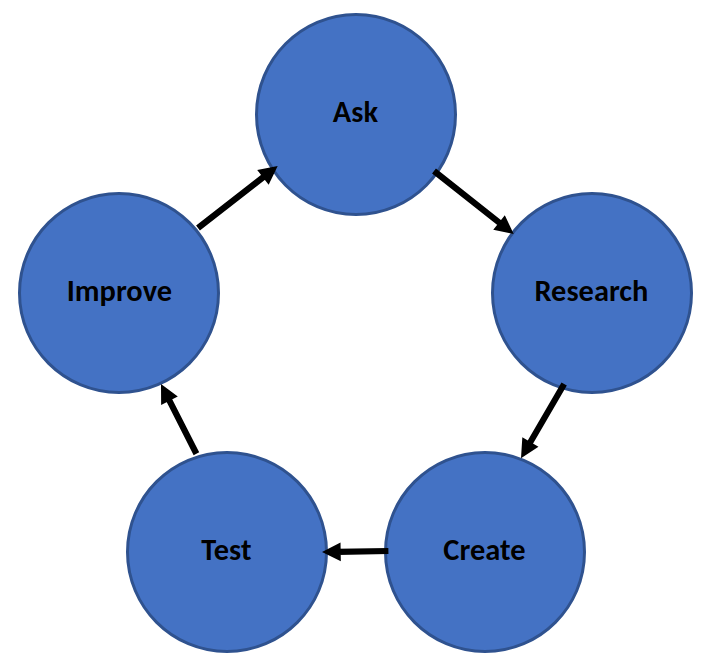
\includegraphics[width=0.99\linewidth]{engineeringCycle.png}
        \end{figure}
    \end{minipage}
	\centering
	\begin{minipage}{0.55\linewidth}
        \begin{figure}
            \centering
            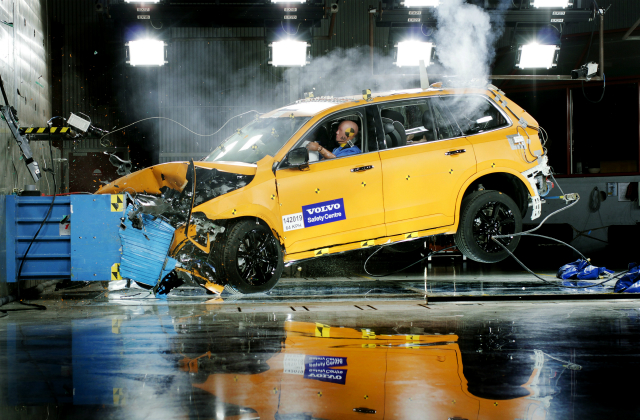
\includegraphics[width=0.99\linewidth]{crash_test.jpg}
        \end{figure}
    \end{minipage}
\end{frame}

\begin{frame}{``New space'' era}
    \begin{itemize}
        \item Space launch startup boom in the last decade
        \item Varying mission parameters
        \begin{itemize}
            \item Payload: satellite, probe, lander, humans
            \item Trajectory: LEO/GTO, translunar, deep space
            \item Capacity: 100 - 150,000 kg to LEO
        \end{itemize}  
        \item Many propulsion configurations
        \begin{itemize}
            \item Solid, bipropellant, hypergolic
            \item (Non-)cryogenic liquid, gaseous propellant 
            \item Injector geometry, flow rates
            \item Gas-generator, expander, tap-off power cycle
        \end{itemize}
        \item Additive manufacturing poised to accelerate and democratize
    \end{itemize}
	\begin{minipage}{0.33\linewidth}
		\begin{figure}
			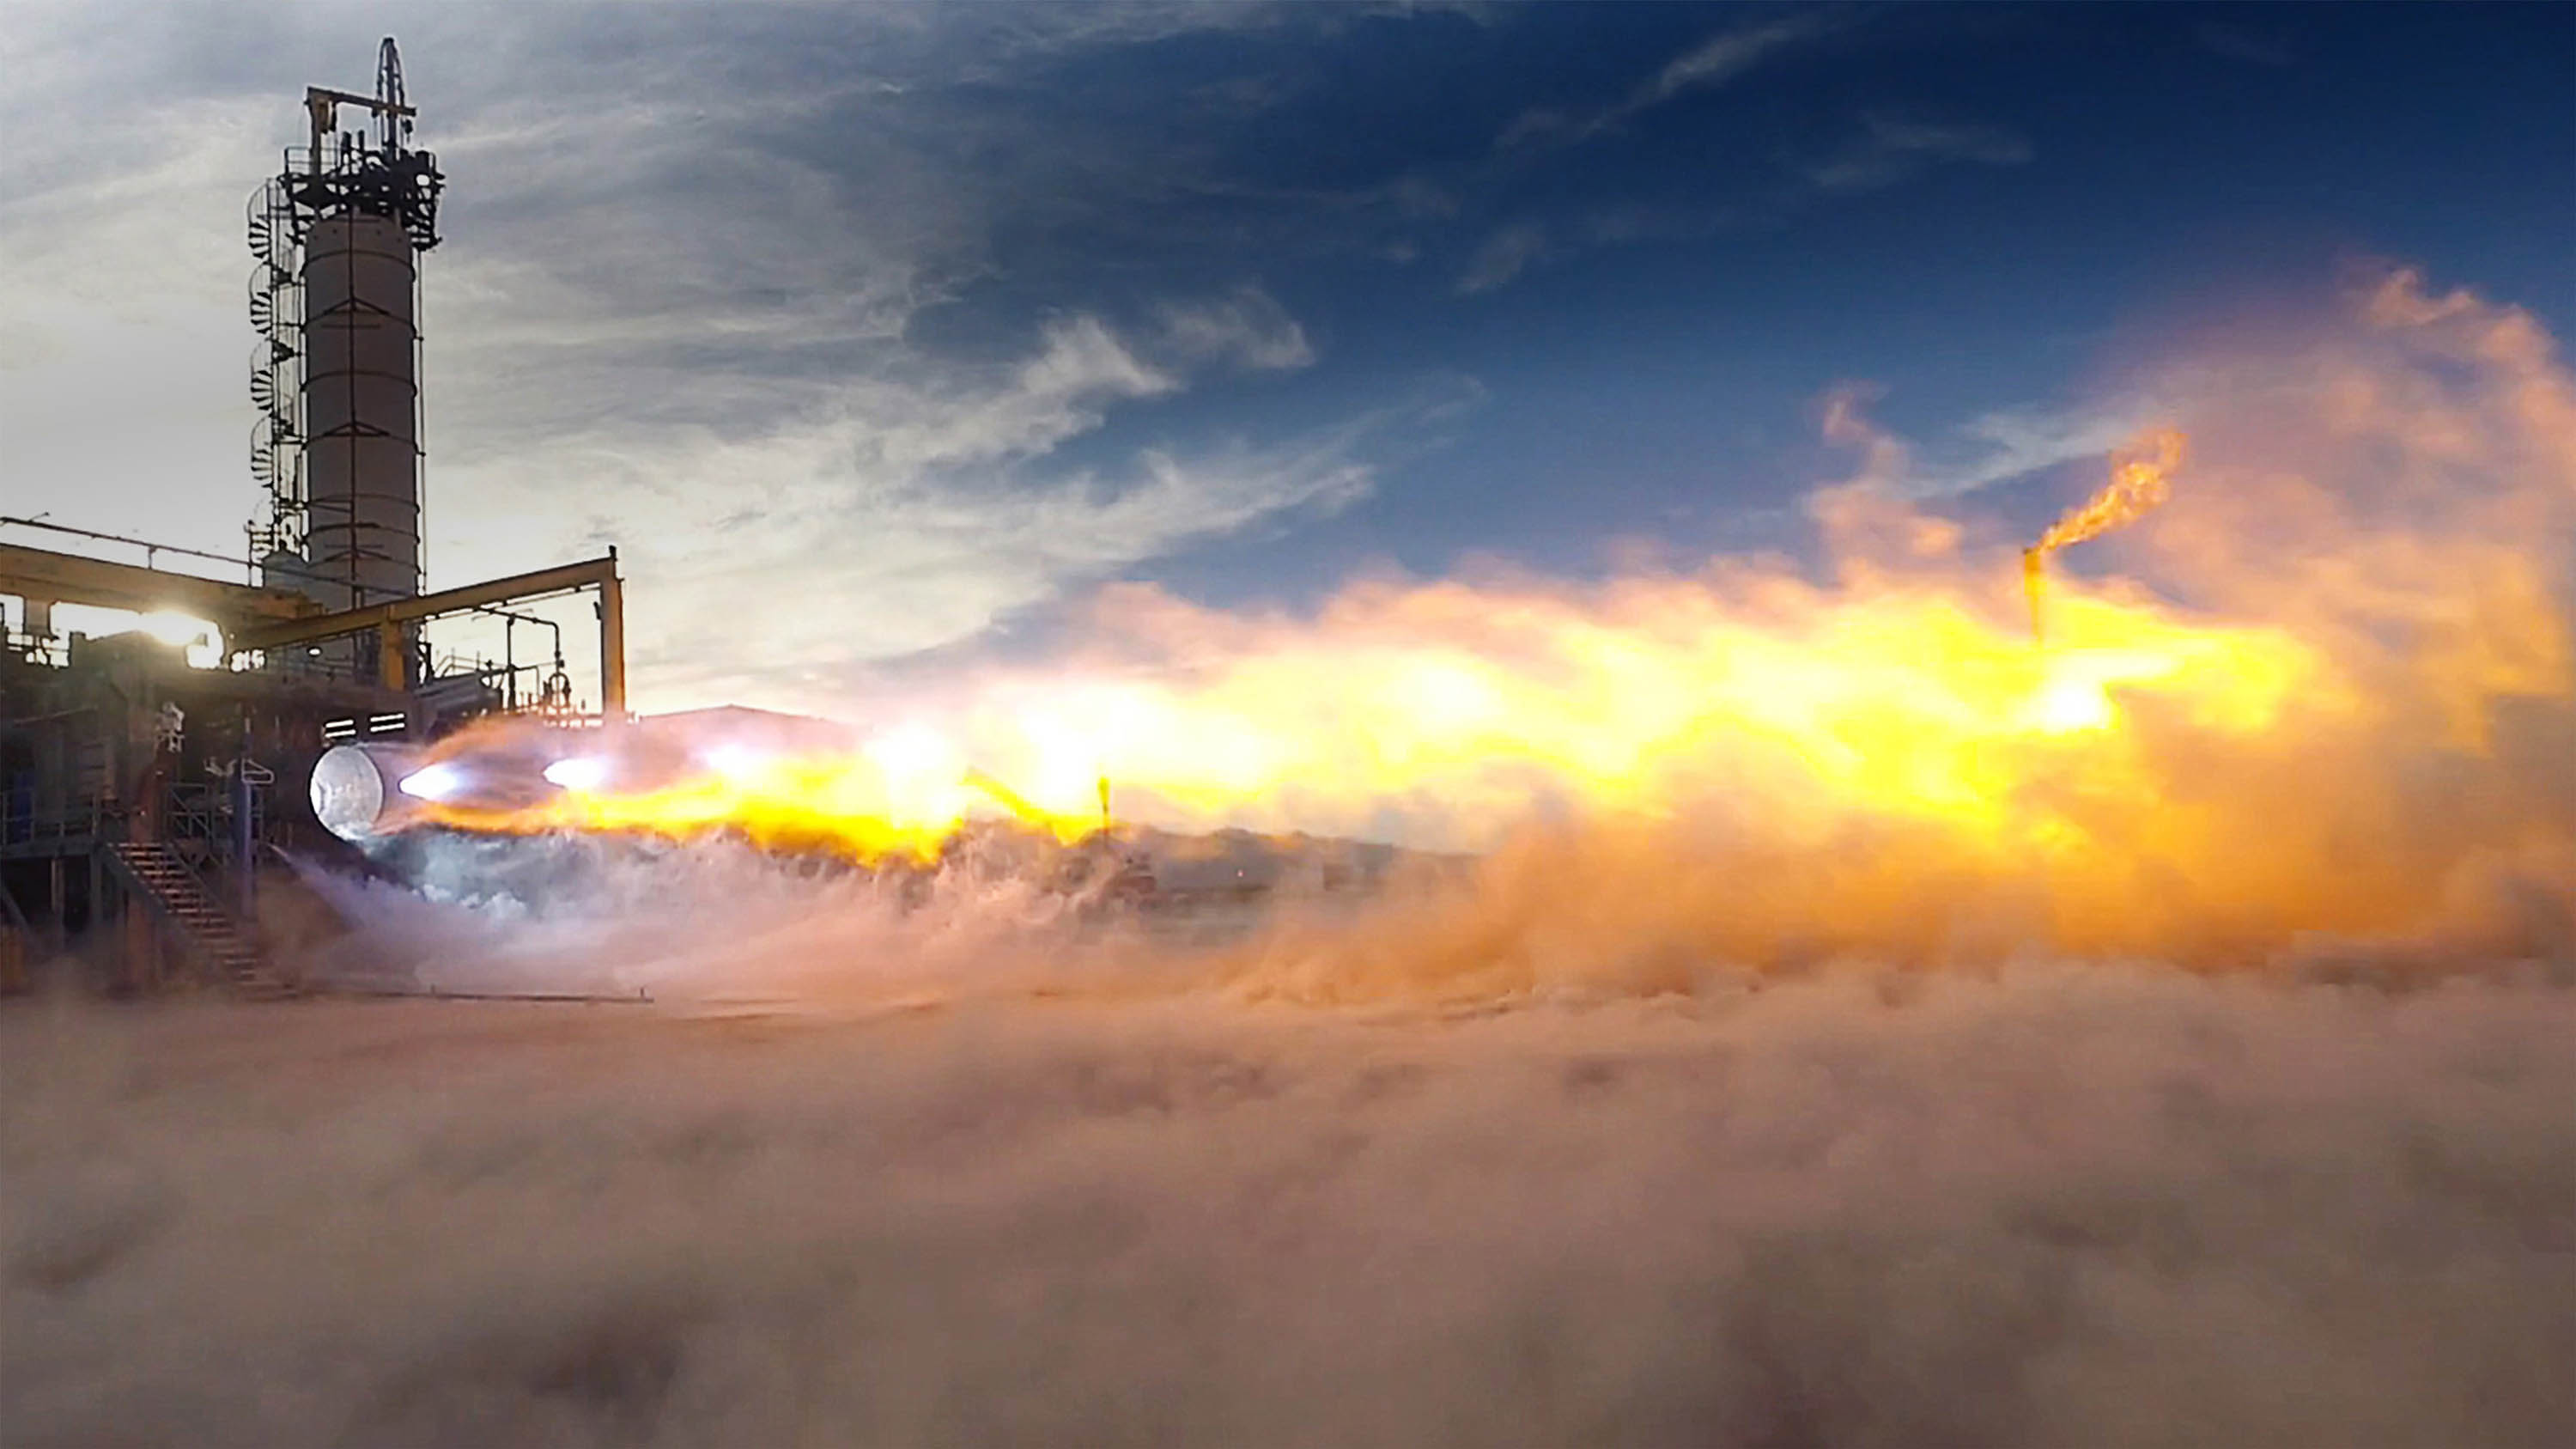
\includegraphics[width=0.99\linewidth]{be4.jpg}
		\end{figure}
	\end{minipage}
	\begin{minipage}{0.33\linewidth}
		\begin{figure}
			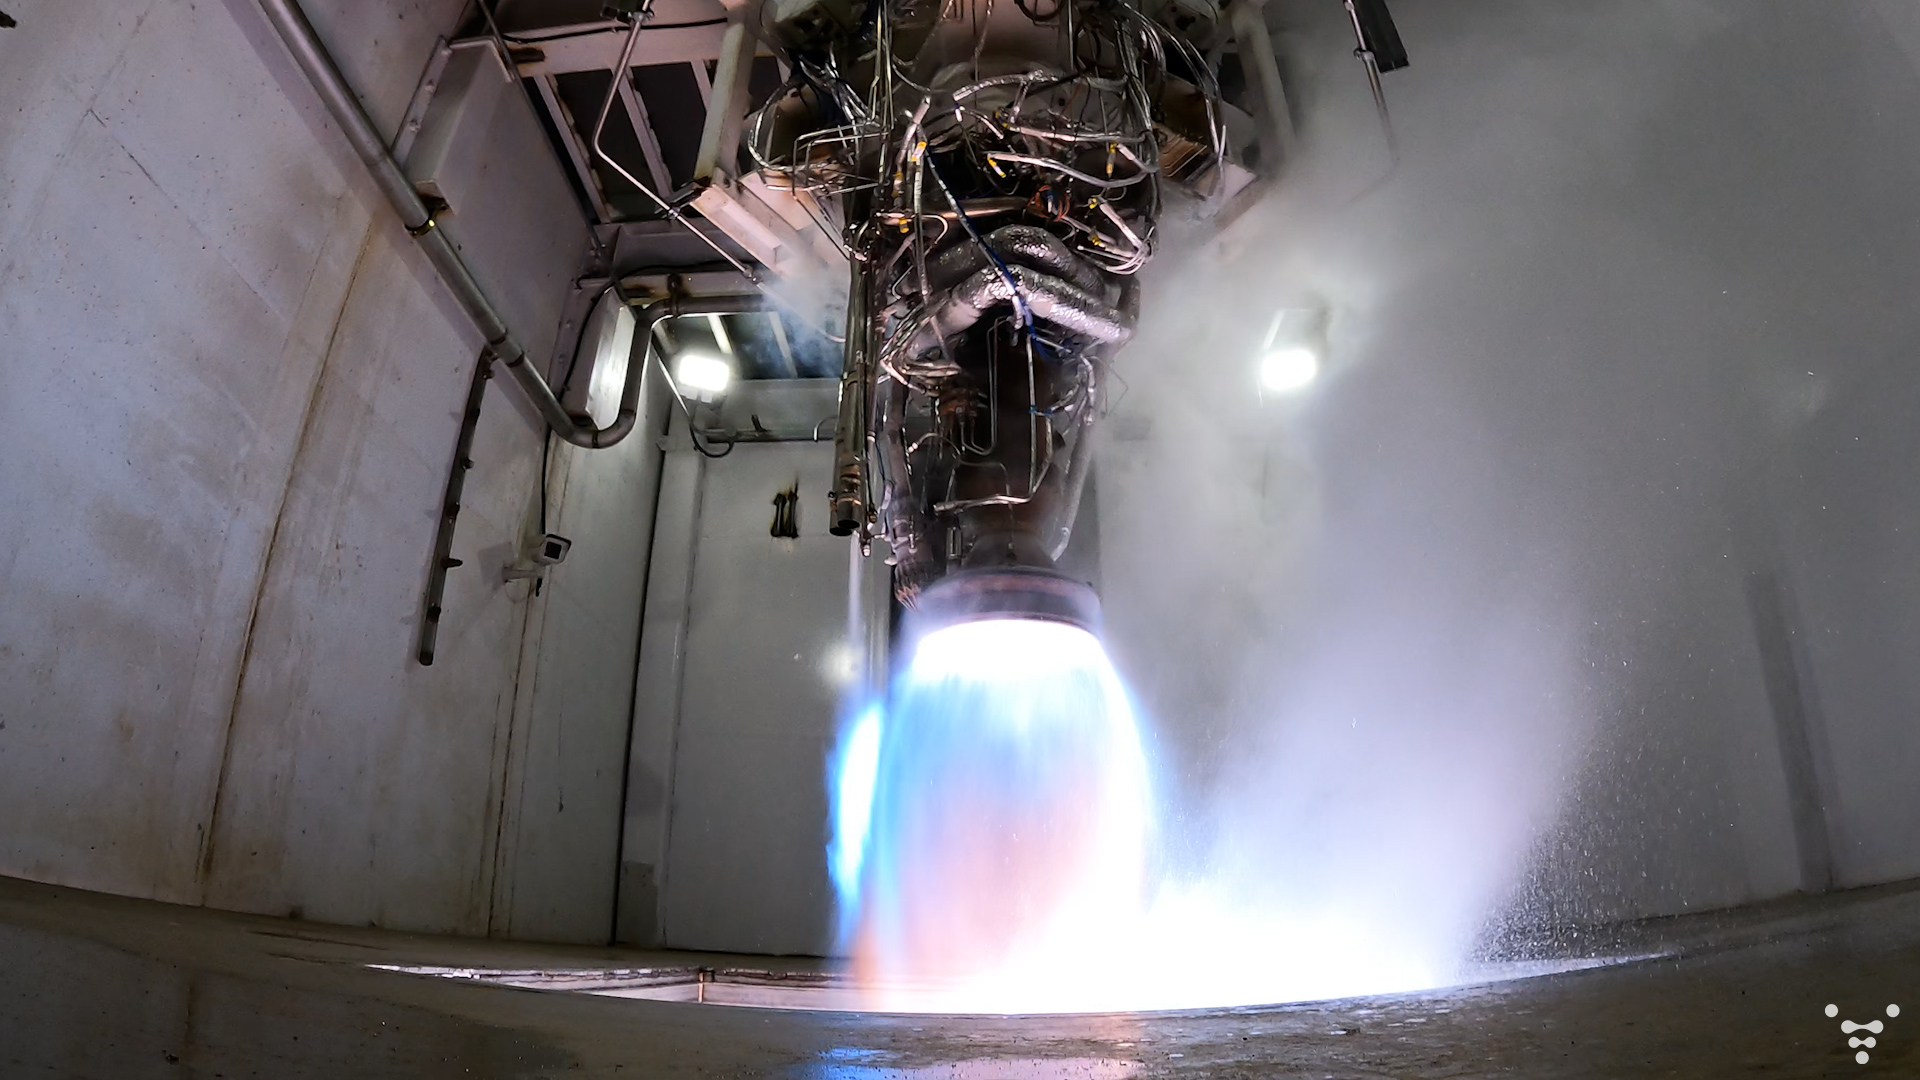
\includegraphics[width=0.99\linewidth]{aeonR.png}
		\end{figure}
	\end{minipage}
	\begin{minipage}{0.28\linewidth}
		\begin{figure}
			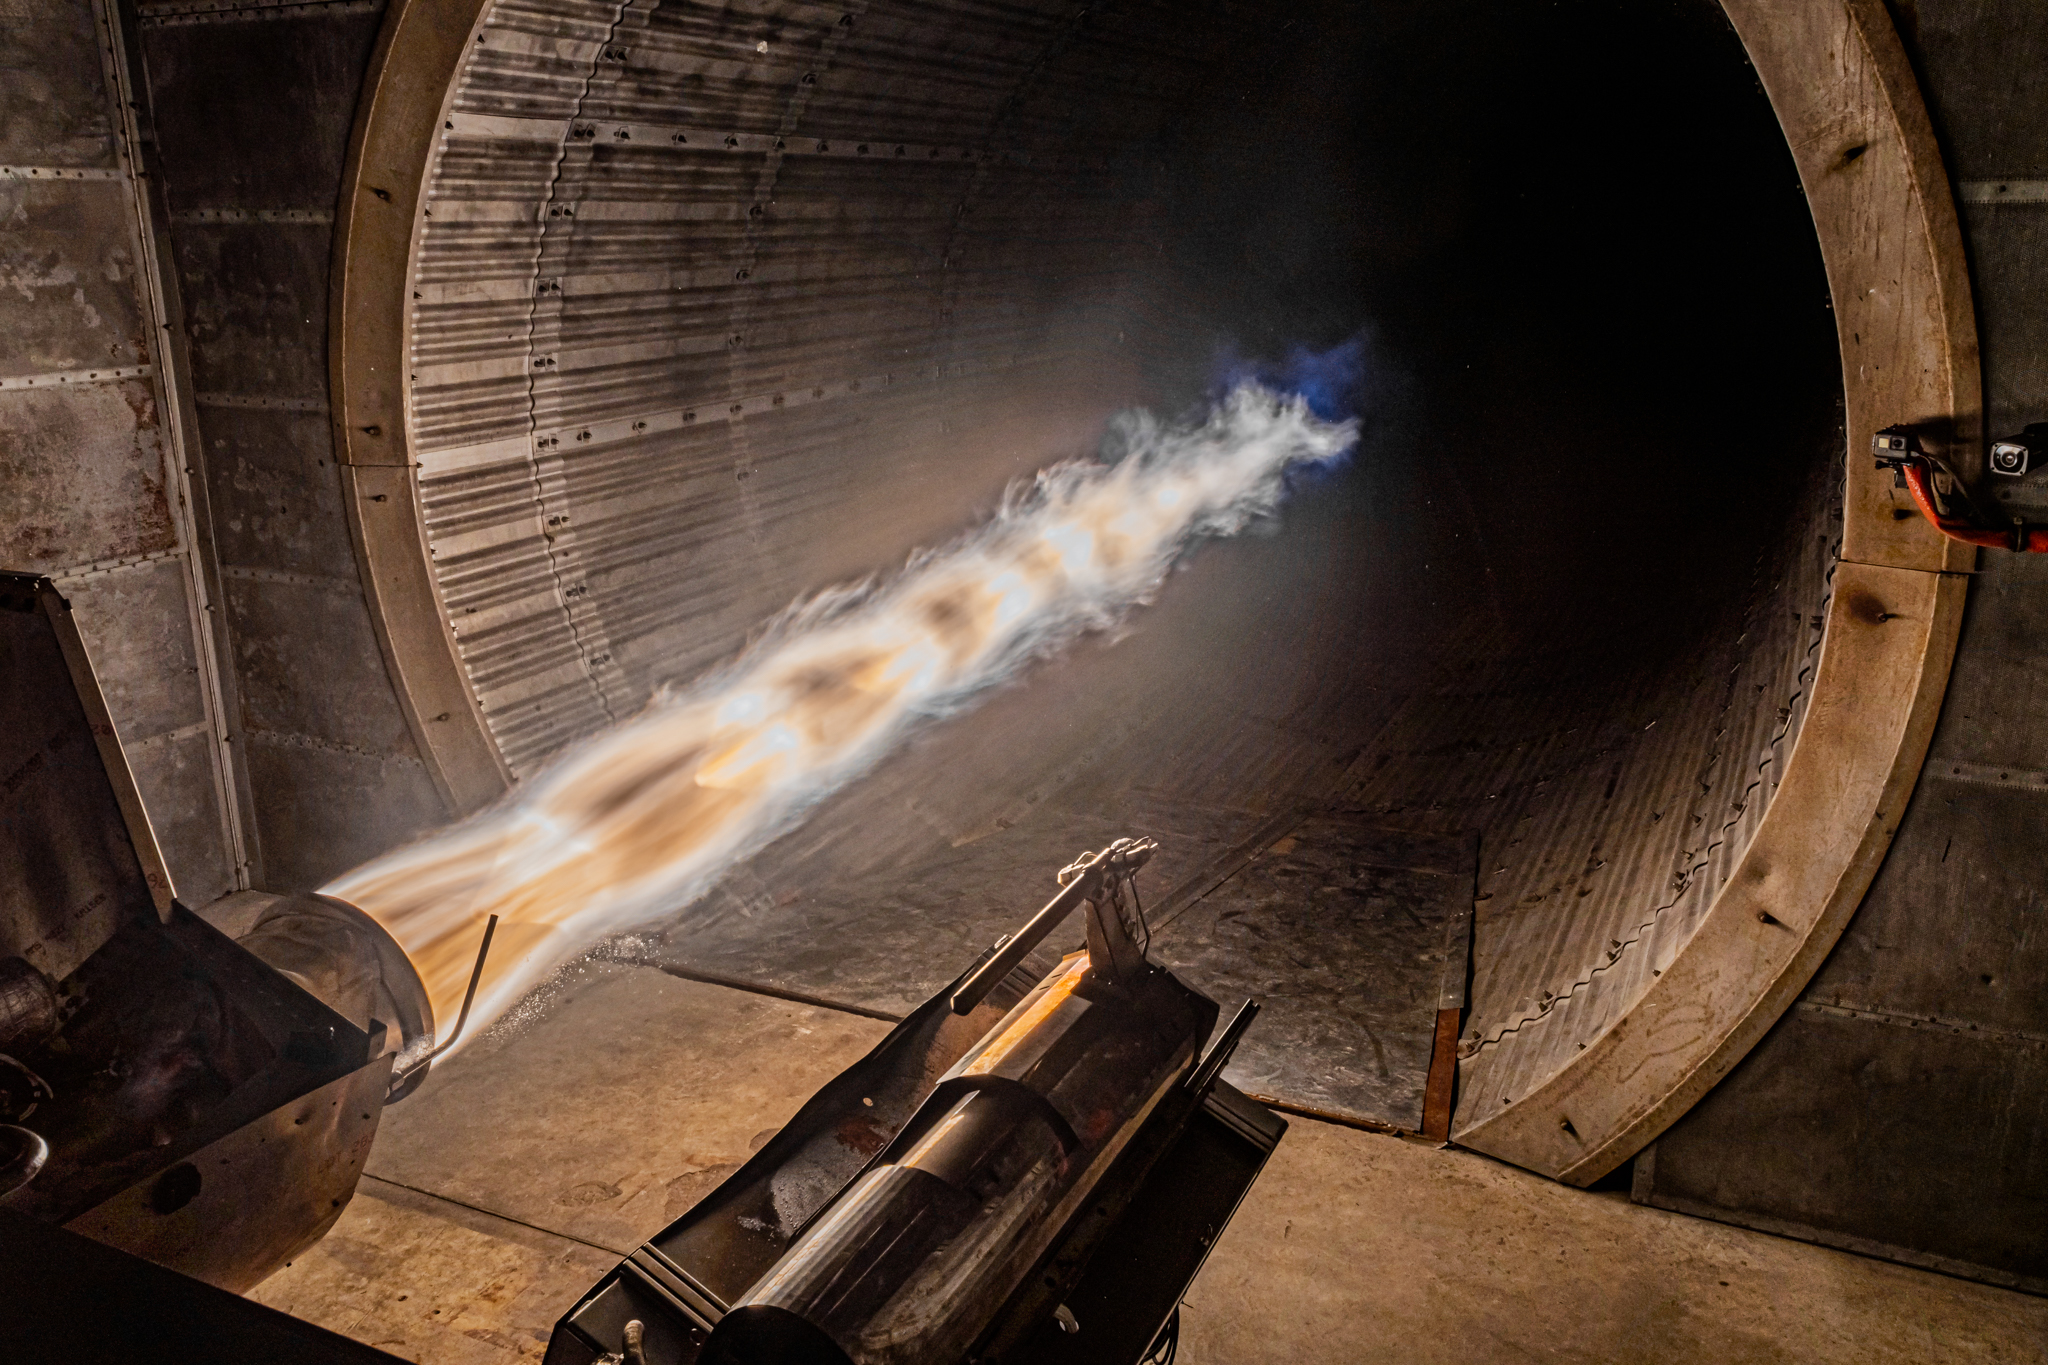
\includegraphics[width=0.99\linewidth]{delphin.jpeg}
		\end{figure}
	\end{minipage}
\end{frame}

\begin{frame}{Cost of experiments (in 2022 USD)}
    \begin{itemize}
        \item Rocketdyne F-1 (Saturn V)
        \begin{itemize}
            \item \$4.8 billion development cost
            \item \$30 million per unit
            \item \$1.6 billion per launch
        \end{itemize}
        \item SpaceX Merlin 1D (Falcon Heavy)
        \begin{itemize}
            \item \$1 million per unit
            \item \$97 million per launch
        \end{itemize}
    \end{itemize}
	\begin{minipage}{0.49\linewidth}
		\begin{figure}
			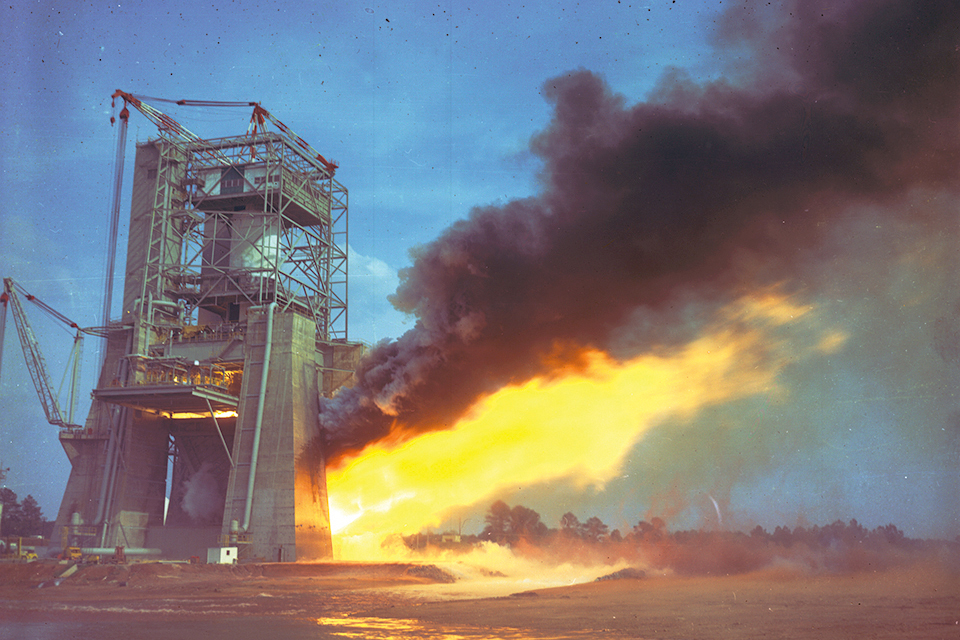
\includegraphics[width=0.99\linewidth]{f1TestStand.jpg}
		\end{figure}
	\end{minipage}
	\begin{minipage}{0.49\linewidth}
		\begin{figure}
			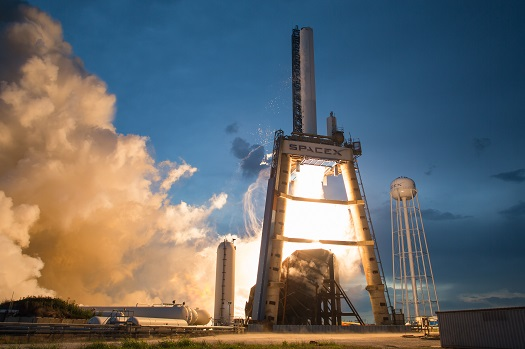
\includegraphics[width=0.99\linewidth]{merlin1dTestStand.jpg}
		\end{figure}
	\end{minipage}
\end{frame}

\begin{frame}{Cost of simulations}
    \begin{itemize}
        \item IBM Summit at ORNL
        \begin{itemize}
            \item $\sim$\$200 million (2019 USD) to design and build
            \item 13 MW peak consumption ($\sim$11,000 homes)
            \item $\sim$\$10 million annual energy cost (overestimated)
        \end{itemize}
        \item Combustion LES/DNS
        \begin{itemize}
            \item $\numDOF \sim \; \text{Re}^{9/4}$
            \item 50+ species, 100+ reactions
            \item $\Delta t = \mathcal{O}(1\text{e-}9 \; s)$
        \end{itemize}
    \end{itemize}
	\centering
	\begin{minipage}{0.3\linewidth}
		\centering
		\begin{figure}
			\centering
			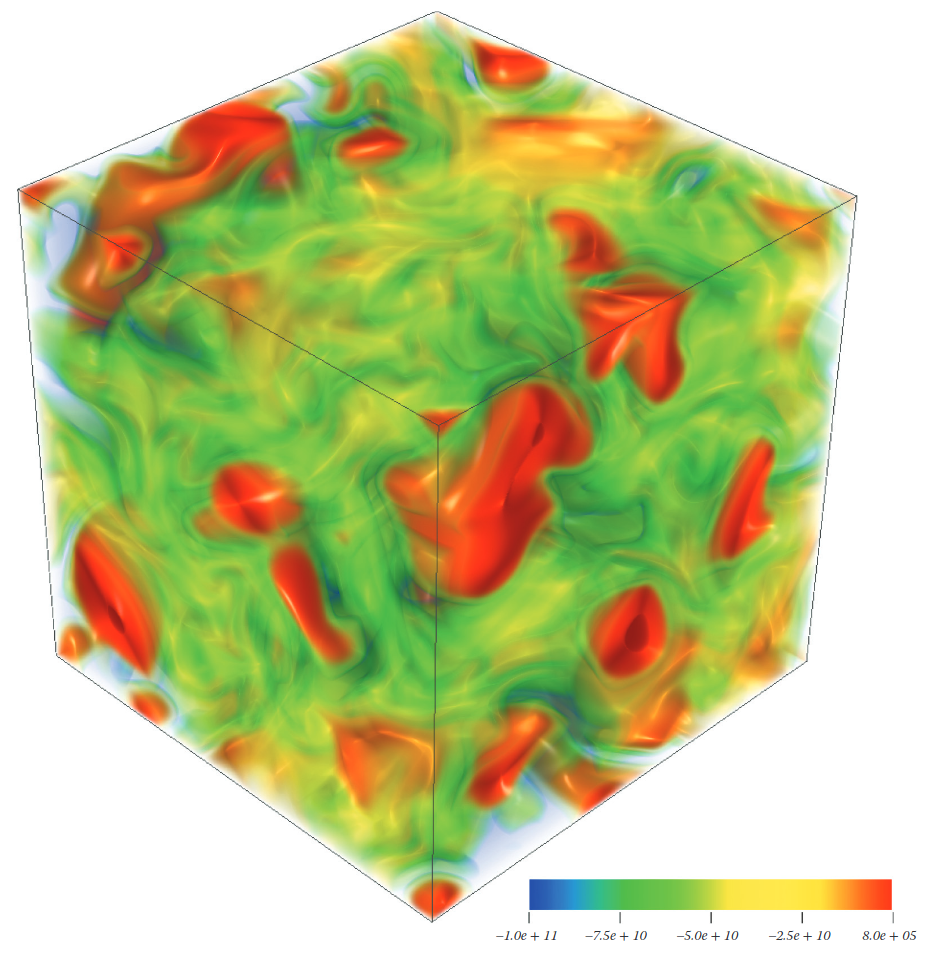
\includegraphics[width=0.95\linewidth]{combustionDNS.png}
		\end{figure}
	\end{minipage}
	\hspace{1cm}
	\centering
	\begin{minipage}{0.3\linewidth}
		\centering
		\begin{figure}
			\centering
			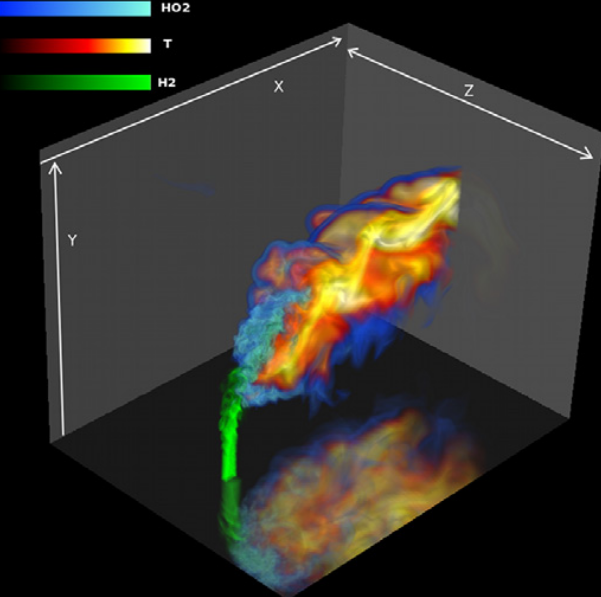
\includegraphics[width=0.95\linewidth]{jetCrossflowDNS.png}
		\end{figure}
	\end{minipage}
	
\end{frame}

\begin{frame}{Data-driven reduced-order models (ROMs)}
	\begin{itemize}
		\item Learning cheap models from high fidelity simulations, experiments
		\item Non-intrusive methods
		\begin{itemize}
			\item Only require system output
			\item Black/gray box models
			\item Kriging, operator inference, ANNs
		\end{itemize}
		\item Intrusive methods
		\begin{itemize}
			\item Directly manipulate governing equations
			\item Galerkin, Petrov--Galerkin projection
		\end{itemize}
	\end{itemize}
\end{frame}

\begin{frame}{Projection-based ROMs of non-linear systems}
    \begin{itemize}
        \item Mapping from low-dim latent space to approximate solution manifold
        \item Map governing equations onto test manifold, evolve in time
    \end{itemize}
	\centering
	\begin{minipage}{0.49\linewidth}
		\centering
		\vspace{-2em}
		\begin{equation*}
			\ode{\stateVec}{\timeVar} = \rhsFunc{\stateVec}
		\end{equation*}
		\begin{equation*}
			\ode{\stateVecCoef}{\timeVar} = \encoderFunc{\rhsFunc{\decoderFunc{\stateVecCoef}}}
		\end{equation*}
	\end{minipage}
	\hspace{-2em}
	\begin{minipage}{0.49\linewidth}
		\begin{figure}
			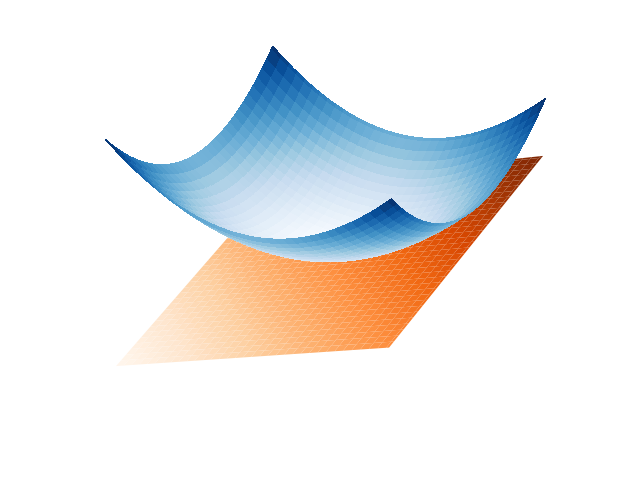
\includegraphics[width=0.99\linewidth,trim={2em 2em 2em 2em},clip]{tangentPlane.png}
		\end{figure}
	\end{minipage}
	\begin{tcolorbox}[colframe=red!50!white,halign=center]
		PROMs of non-linear systems have \textbf{no stability guarantees} \\
		Accuracy/robustness are rarely tested beyond canonical problems
	\end{tcolorbox}
\end{frame}

\begin{frame}{Contributions}
    \begin{enumerate}
        \item Assessment and improvement of state-of-the-art PROMs for practical CFD systems (e.g. 2D transonic cavity and 3D rocket combustor)
        \item Improved solution/RHS formulation of hyper-reduced MP-LSVT method with enhanced accuracy and robustness
        \item Memory- and compute-scalable HPROM framework in high-performance combustion CFD code
        \item Open-source toolchain for pre- and post-processing of HPROMs for very large CFD datasets
        \item End-to-end analysis of the computational cost, accuracy, and robustness of sparse-sampling hyper-reduction methods
        \item The first study of PROMs for a 3D multi-injector rocket combustor, containing 250 million DOFs
        \item PERFORM, an open-source Python package for rapid prototyping of novel ROM methods
    \end{enumerate}
\end{frame}

\section*{Projection ROMs}

\begin{frame}{Projection-based ROMs}
    \begin{itemize}
		\item General non-linear ODE
		\begin{equation*}
			\ode{\consVec}{\timeVar} + \rhsFunc{\consVec} = \zeroVec \quad \consVec \in \mathbb{R}^{\numDOF}
		\end{equation*}
			\item Low-dimensional affine representation ($\numConsvModes \ll \numDOF$)
		\begin{align*}
			\consVec(\timeVar) \approx \consVecRom(\timeVar) &\triangleq \consVecCent + \consScale \sum^{\numConsvModes}_{i=1} \consVarCoef(\timeVar) \consTrialVec \\
			&= \consVecCent + \consScale \consTrial \consVecCoef(\timeVar)
		\end{align*}
		\begin{equation*}
			\consVecCoef \in \mathbb{R}^{\numConsvModes}, \; \consTrial \in \mathbb{R}^{\numDOF \times \numConsvModes}
		\end{equation*}
		\item Centering profile $\consVecCent$ and scaling matrix $\consScale$ are crucial; more later
		\begin{equation*}
			\consScale \triangleq \text{diag}\left( \consScaleVar_1, \, \consScaleVar_2, \, \hdots, \, \consScaleVar_{\numDOF} \right)
		\end{equation*}
	\end{itemize}
\end{frame}

\begin{frame}{The trial basis}
    \begin{itemize}
        \item The proper orthogonal decomposition (POD)
        \begin{equation*}
            \consTrial = \argmin{\dummyMatOne \in \mathbb{R}^{\numDOF \times \numConsvModes}} \norm{\consDataMat - \dummyMatOne \dummyMatOne^\top \consDataMat}_2^2
        \end{equation*}
        \begin{equation*}
            \consDataMat = \basisMat \singVecMat \rightSingVecMat^\top, \quad \consTrial \leftarrow \basisMat[:, {:}\numConsvModes]
        \end{equation*}
    \end{itemize}
	\vspace{-1em}
	\centering
	\begin{figure}
		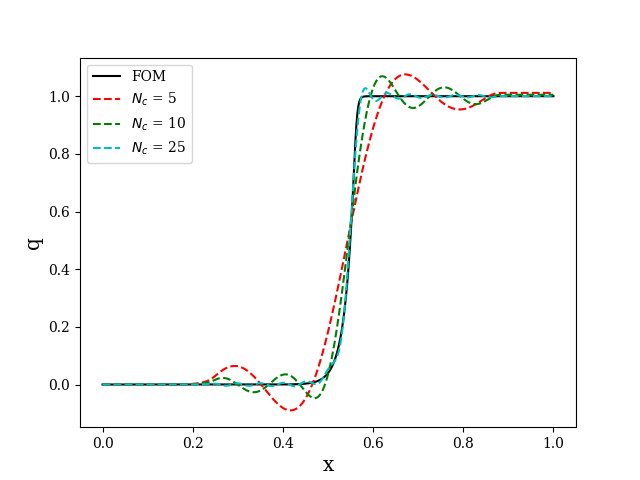
\includegraphics[width=0.6\linewidth]{podProfileConverge.png}
	\end{figure}
\end{frame}

\begin{frame}{The test basis}
    \begin{itemize}
        \item Inserting approximation, no order reduction yet
        \begin{equation*}
            \consScale \consTrial \ode{\consVecCoef}{\timeVar} + \rhsFunc{\consVecCent + \consScale \consTrial \consVecCoef} = \zeroVec 
        \end{equation*}
        \item Project via test basis $\testBasis \in \mathbb{R}^{\numDOF \times \numConsvModes}$, rearrange
        \begin{equation*}
            \ode{\consVecCoef}{\timeVar} + \left[ \testBasis^\top \consScale \consTrial \right]^{-1} \testBasis^\top \rhsFunc{\consVecRom} = \zeroVec
        \end{equation*}
        \item $\testBasis = \consTrial$: Galerkin projection
        \item $\testBasis \neq \consTrial$: Petrov--Galerkin projection 
    \end{itemize}
\end{frame}

\begin{frame}{Least-squares Petrov--Galerkin (LSPG)}
    \begin{itemize}
		\item Fully-discrete residual (e.g. BDF1)
		\begin{equation*}
			\resFuncIter{\timeIdx}{\consVecCoef^{\newtonIdx}} \triangleq \consScale \consTrial \left( \consVecCoef^{\newtonIdx} - \consVecCoef^{\timeIdx-1} \right) + \dt \, \rhsFunc{\consVecCent + \consScale \consTrial \consVecCoef^{\newtonIdx}} = \zeroVec
		\end{equation*}
		\item Minimize with Gauss--Newton
		\begin{equation*}
			\consVecCoef^{\timeIdx} = \argmin{\dummyVec \in \mathbb{R}^{\numConsvModes}} \norm{\resFuncIter{\timeIdx}{\dummyVec}}_2^2
		\end{equation*}
		\begin{equation*}
			\delta \consVecCoef^{\newtonIdx, \timeIdx} = \argmin{\dummyVec \in \mathbb{R}^{\numConsvModes}} \norm{\pde{\resFuncIter{\timeIdx}{\dummyVec}}{\dummyVec} \dummyVec + \resFuncIter{\timeIdx}{\dummyVec}}_2^2
		\end{equation*}
		\item Equivalent to Petrov--Galerkin projection with test basis
		\begin{equation*}
			\testBasis = \pde{\resFuncIter{\timeIdx}{\consVecCoef^{\newtonIdx}}}{\consVec} \consScale \consTrial
		\end{equation*}
	\end{itemize}
\end{frame}

\begin{frame}{Model-preserving least-squares with variable transformation}
    \begin{itemize}
		\item Conservative variables are cumbersome in multi-physics simulations
		\item Choose alternative (complete) set of variables, e.g. primitive variables
		\begin{equation*}
			\stateVar_p \triangleq \left[ p, \; u_i, \; T, \; Y_l \right]
		\end{equation*}
		\begin{equation*}
			\primVecRom(\timeVar) \triangleq \primVecCent + \primScale \primTrial \primVecCoef(\timeVar)
		\end{equation*}
		\item Frame residual in terms of primitive state
		\begin{equation*}
			\resFuncIter{\timeIdx}{\primVecCoef^{\newtonIdx}} \triangleq \consFunc{\primVecCent + \primScale \primTrial \primVecCoef^{\newtonIdx}} - \consVec^{\timeIdx-1} + \dt \, \rhsFunc{\primVecCent + \primScale \primTrial \primVecCoef^{\newtonIdx}} = \zeroVec
		\end{equation*}
		\item Gauss--Newton w/r/t \textbf{primitive} modal coefficients
		\begin{equation*}
			\testBasis = \pde{\resFuncIter{\timeIdx}{\primVecCoef^{\newtonIdx}}}{\primVec} \primScale \primTrial
		\end{equation*}
	\end{itemize}
\end{frame}

\section*{Hyper-reduction}

\begin{frame}{The lifting bottleneck}
    \begin{itemize}
		\item Non-linear terms $\rhsFunc{\primVecRom}$ still scale with full dimension $\numDOF$
		\item For same time integrator and \dt, ROM is usually \textbf{more} expensive
		\item Can we approximate non-linear terms from a few samples?
		\begin{equation*}
			\rhsFunc{\primVec} \approx \sampFunc{\sampMat \rhsFunc{\primVec}}, \quad \sampMat \in \mathbb{R}^{\numSamps \times \numDOF}
		\end{equation*}
	\end{itemize}
	\vspace{1em}
	\begin{figure}
		\centering
		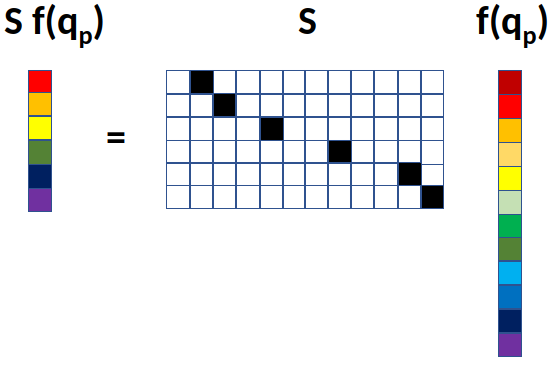
\includegraphics[width=0.55\linewidth]{samplingHelperVis.png}
	\end{figure}
\end{frame}

\begin{frame}{Least-squares regression \& interpolation}
    \begin{itemize}
		\item Approximate non-linear terms with POD basis $\deimBasisRes \in \mathbb{R}^{\numDOF \times \numResModes}$
		\begin{align*}
			\resFunc{\primVecCoef} \approx \resApproxFunc{\primVecCoef} &= \deimBasisRes \dummyVec \\
			\sampMat \resApproxFunc{\primVecCoef} &= \sampMat \deimBasisRes \dummyVec
		\end{align*}
		\item Gappy POD ($\numSamps > \numResModes$)
		\begin{equation*}
			\resApproxFunc{\primVecCoef} \triangleq \deimBasisRes \left[ \sampMat \deimBasisRes \right]^{+} \sampMat \resFunc{\primVecCoef}
		\end{equation*}
		\item Discrete empirical interpolation method ($\numSamps = \numResModes$)
		\begin{equation*}
			\resApproxFunc{\primVecCoef} \triangleq \deimBasisRes \left[ \sampMat \deimBasisRes \right]^{-1} \sampMat \resFunc{\primVecCoef}
		\end{equation*}
	\end{itemize}
\end{frame}

\begin{frame}{Sampling algorithms}
    
\end{frame}

\begin{frame}{Separate regression basis formulation}
    \begin{itemize}
		\item Hyper-reduction of residual function has several drawbacks
		\begin{itemize}
			\item FOM and ROM non-linear solver are never the same
			\item Enormous range of scales during convergence, $\mathcal{O}(1\text{e-}3)-\mathcal{O}(1\text{e-}12)$
			\item Train from first, last, all subiterations?
		\end{itemize}
		\item Approximate time integrator and RHS separately
		\begin{align*}
			\consFuncRom{\primVec} &\triangleq \deimRegressorCons \consFunc{\primVec} \\
			\rhsApproxFunc{\primVec} &\triangleq \deimRegressorRhs \rhsFunc{\primVec}
		\end{align*}
		\begin{equation*}
			\resApproxFuncIter{\timeIdx}{\primVecCoef^{\newtonIdx}} \triangleq \consFuncRom{\primVecRom^{\newtonIdx}} - \consFuncRom{\primVecRom^{\timeIdx}} + \dt \, \rhsApproxFunc{\primVecRom^{\timeIdx}} = \zeroVec
		\end{equation*}
	\end{itemize}
\end{frame}

\begin{frame}{Separate regression basis formulation}
	\vspace{-1.9em}
	\begin{align*}
		\delta \primVecCoef^{\newtonIdx} = \underset{\dummyVec \in \mathbb{R}^{\numPrimModes}}{argmin} \Bigg\lVert \bigg(\deimBasisCons \underbrace{\deimRegressorConsTiny \sampMat \pde{\consVec^{\newtonIdx}}{\primVec} \primScale \primTrial }_{\dummyMatOne} - \deimBasisRhs \underbrace{\deimRegressorRhsTiny \sampMat \, \dt \, \pde{\rhsVec^{\newtonIdx}}{\primVec} \primScale \primTrial}_{\dummyMatTwo} \bigg) \dummyVec \\
		+ \deimBasisCons \underbrace{\deimRegressorConsTiny \sampMat \left( \consVec(\primVecRom^{\newtonIdx}) - \consVec(\primVecRom^{\newtonIdx}) \right)}_{\dummyVecOne} - \deimBasisRhs \underbrace{\deimRegressorRhsTiny \sampMat \rhsFunc{\primVecRom^{\newtonIdx}}}_{\dummyVecTwo} \Bigg\rVert_2^2
	\end{align*}
	\vspace{-1em}
	\begin{itemize}
		\item Normal equations
		\begin{align*}
			\left(\dummyMatOne^\top \dummyMatOne - \dummyMatOne^\top \deimBasisCons^\top \deimBasisRhs \dummyMatTwo - \dummyMatTwo^\top \deimBasisRhs^\top \deimBasisCons \dummyMatOne + \dummyMatTwo^\top \dummyMatTwo \right) \delta \primVecCoef^{\newtonIdx} \\
			= -\left(\dummyMatOne^\top \dummyVecOne - \dummyMatOne^\top \deimBasisCons^\top \deimBasisRhs \dummyVecTwo - \dummyMatTwo^\top \deimBasisRhs^\top \deimBasisCons \dummyVecOne + \dummyMatTwo^\top \dummyVecTwo\right)
		\end{align*}
		\item Precomputed:
		\begin{itemize}
			\item $\deimRegressorConsTiny \in \mathbb{R}^{\numConsvModes \times \numSamps}$
			\item $\deimRegressorRhsTiny \in \mathbb{R}^{\numRHSModes \times \numSamps}$
			\item $\deimBasisRhs^\top \deimBasisCons \in \mathbb{R}^{\numRHSModes \times \numConsvModes}$
		\end{itemize}
	\end{itemize}
\end{frame}

\section*{Numerical Experiments}

\begin{frame}{Numerical Experiments}
    \begin{itemize}
		\item The General Equations and Mesh Solver (GEMS)
		\begin{itemize}
			\item 2nd-order unstructured finite volume
			\item BDF2 time integration w/ pseudo time-stepping
			\item Finite-rate and flamelet-progress variable chemistry models
		\end{itemize}
		\item Compressible Navier--Stokes equations with scalar transport
	\end{itemize}
	\begin{equation*}
		\pde{\consVec}{\timeVar} + \nabla \cdot (\invFluxDir - \viscFluxDir) = \sourceVec
	\end{equation*}
	\scriptsize
	\def\arraystretch{2}
	\begin{equation*}
		\consVec = \left[
		\begin{array}{c}
		\rho \\ \rho u \\ \rho v \\ \rho w \\ \rho h^0 - p \\ \hdashline[2pt/2pt] \rho Y_{\specIdx} \\
		\end{array}
		\right]  \; \;
		\invFluxDir = \left[
		\begin{array}{c}
		\rho u_i \\  \rho uu_i + \delta_{xi} p \\ \rho vu_i + \delta_{yi} p \\ \rho wu_i + \delta_{zi} p \\ \rho h^0 u_i \\ \hdashline[2pt/2pt] \rho Y_{\specIdx} u_i 
		\end{array}
		\right]  \; \;
		\viscFluxDir = \left[
		\begin{array}{c}
		0 \\ \tau_{ix} \\ \tau_{iy} \\ \tau_{iz} \\ u_j \tau_{ji} - q_i \\ \hdashline[2pt/2pt] \rho D  \pde{Y_{\specIdx}}{x_i}
		\end{array}
		\right]  \; \;
		\mathbf{s} = \left[
		\begin{array}{c}
		0 \\ 0 \\ 0 \\ 0 \\ 0 \\ \hdashline[2pt/2pt] \dot{\omega}
		\end{array} \right]
	\end{equation*}
	\normalsize
\end{frame}

\begin{frame}{2D transonic flow over open cavity}
    
\end{frame}

\begin{frame}{3D truncated CVRC}
    
\end{frame}

\begin{frame}{3D nine-element combustor}
    
\end{frame}

\section*{Miscellaneous}

\begin{frame}{PERFORM}
    % picture of API
    % hierarchy of test cases
    % uses (Elnaz, Wayne, 577 students)
\end{frame}

\begin{frame}{HPROM toolchain (contribution to PDP)}
    % make sure to emphasize that this is Nick's
    % Method of snapshots, sampling, projection/regression error
\end{frame}

\section*{Conclusions}

\begin{frame}{Contributions}
    \begin{enumerate}
        \item Assessment and improvement of state-of-the-art PROMs for practical CFD systems (e.g. 2D transonic cavity and 3D rocket combustor)
        \item Improved solution/RHS formulation of hyper-reduced MP-LSVT method with enhanced accuracy and robustness
        \item Memory- and compute-scalable HPROM framework in high-performance combustion CFD code
        \item Open-source toolchain for pre- and post-processing of HPROMs for very large CFD datasets
        \item End-to-end analysis of the computational cost, accuracy, and robustness of sparse-sampling hyper-reduction methods
        \item The first study of PROMs for a 3D multi-injector rocket combustor, containing 250 million DOFs
        \item PERFORM, an open-source Python package for rapid prototyping of novel ROM methods
    \end{enumerate}
\end{frame}

\begin{frame}{Publications and presentations}
	\begin{itemize}
		\item Journal articles
		\vspace{0.5em}
		\begin{itemize}
			\item \tiny \textbf{Wentland, C.R.}, Huang, C., and Duraisamy, K., ``Efficient Projection-based Reduced-order Models for Large Multi-scale Fluid Systems,'' in preparation.
			\item \textbf{Wentland, C.R.} and Duraisamy, K., ``PERFORM: A Python package for developing reduced-order models for reacting fluid flows,'' Under review, \textit{J. Open Source Softw.}, https://github.com/cwentland0/perform.
			\item Huang, C., \textbf{Wentland, C.R.}, Duraisamy, K., and Merkle, C., ``Model reduction for multi-scale transport problems using model-form preserving least-squares projections with variable transformation,'' \textit{J. Comp. Phys.}, 2021, Vol. 448, 2021.
        	\item Parish, E.J., \textbf{Wentland, C.R.}, Duraisamy, K., ``The Adjoint Petrov--Galerkin method for non-linear model reduction,'' \textit{Comput. Method Appl. M.}, Vol. 365, 2020.
		\end{itemize}
		\item \normalsize Conference proceedings
		\vspace{0.5em}
		\begin{itemize}
			\item \tiny \textbf{Wentland, C.R.}, Huang, C., and Duraisamy, K., ``Investigation of Sampling Strategies for Reduced-Order Models of Rocket Combustors,'' \textit{AIAA Scitech Forum}, 2021.
			\item \textbf{Wentland, C.R.}, Huang, C., and Duraisamy, K., ``Closure of Reacting Flow Reduced-Order Models via the Adjoint Petrov-Galerkin Method,'' \textit{AIAA Aviation Forum}, 2019.
		\end{itemize}
		\item \normalsize Conference presentations
		\vspace{0.5em}
		\begin{itemize}
			\item \tiny \textbf{Wentland, C.R.} and Duraisamy, K., ``Intrusive and Non-intrusive Non-linear Reduced-order Models for Reacting Flows,'' \textit{2021 Annual Meeting of the APS Division of Fluid Dynamics}, Phoenix, AZ, USA.
			\item \textbf{Wentland, C.R.}, Nair, A.S., and Duraisamy, K., ``Nonlinear Manifold Reduced-Order Models for Complex Fluid Flow Systems,'' \textit{2021 SIAM Conference on Computational Science and Engineering}, virtual.
			\item \tiny \textbf{Wentland, C.R.}, Parish, E.J., and Duraisamy, K., ``Closure of Reduced-Order Models Using Statistical Mechanics Approaches,'' \textit{2018 World Congress on Computational Mechanics}, New York, NY, USA.
		\end{itemize}
	\end{itemize}
	
\end{frame}

\begin{frame}{Future work}
	\begin{itemize}
		\item Complete investigation of nine-element combustor
		\item Implementation of efficient ScaLAPACK/PETSc NLLS solves
		\item Comparison of full residual vs. component-based hyper-reduction
		\item Thorough exploration of effects of feature scaling
		\item Memory-scalable adaptive basis and sampling in GEMS
	\end{itemize}
\end{frame}

\begin{frame}{Acknowledgements}
	\begin{itemize}
	    \item Financial support from the US Air Force Office of Scientific Research through the Center of Excellence Grant FA9550-17-1-0195
	    \item Compute support from the US Department of Defense High Performance Computing Modernization Program
		\item Compute support of ConFlux and Lighthouse systems from the University of Michigan Advanced Research Computing division
		\item Nicholas Arnold-Medabalimi for development and maintenance of the Parallel Data Processing toolbox
	\end{itemize}
	\begin{minipage}{0.36\linewidth}
		\begin{figure}
			
\includegraphics[width=0.99\linewidth,trim={0em 3cm 0em 3cm},clip]{afosr.jpg}
		\end{figure}
	\end{minipage}
	\begin{minipage}{0.3\linewidth}
		\begin{figure}
			
\includegraphics[width=0.99\linewidth]{hpcmp.png}
		\end{figure}
	\end{minipage}
	\begin{minipage}{0.3\linewidth}
		\begin{figure}
			
\includegraphics[width=0.99\linewidth,trim={0em 3cm 0em 3cm},clip]{arc.png}
		\end{figure}
	\end{minipage}
\end{frame}

\end{document}
